\chapter{\'Etale cohomology for schemes} \label{chapter: etale_cohomology_1}
    \begin{abstract}
        Galois theory via algebraic topology ? Game on!
    \end{abstract}
    
    \minitoc
    
    \section{Pr\'elude: Primes in integral extensions}
        \subsection{Behaviours of prime ideals in integral extensions}
            \subsubsection{Finite and integral extensions}
                \begin{definition}[Integral extensions] \label{def: integral_extensions} \index{Integral! extensions} \index{Integral! elements}
                    \noindent
                    \begin{enumerate}
                        \item \textbf{(Integral elements):} Let $A$ be a subring of a commutative ring $B$ (i.e. let their exist monic ring homomorphisms from $A$ to $B$). An element $b \in B$ will be called \textbf{integral} over $A$ if and only if $A[b]$ is a finitely generated commutative $A$-algebra; otherwise, it is called \textbf{transcendental}. When $A$ is a field, what one recovers are the notions of algebraic and transcendental elements (for instance, $\sqrt{2}$ is integral over $\Z$, as it is algebraic over $\Q$, whereas a formal variable $x$ is neither). 
                        \item \textbf{(Integral extensions):} A homomorphism between commutative rings $A \to B$ will be called an integral extension if all elements of $B$ are integral over $B$. Alternatively (and perhaps less confusingly), one may view an integral extension of a commutative ring $A$ as a tensor product $\bigotimes_{i \in I} A[b_i]$ wherein $\{b_i\}_{i \in I}$ is a (possibly infinite) set of elements that are integral over $A$; note that one has the following canonical isomorphism of commutative $A$-algebras:
                            $$\bigotimes_{i \in I} A[b_i] \cong A\left[\{b_i\}_{i \in I}\right]$$
                        thanks to the fact that left-adjoints (the polynomial ring free construction) commutes with colimits (tensor products of commutative algebras). Additionally, integral extensions are trivially injective ring homomorphisms.
                        \item \textbf{(Integral closures):} Let $\varphi: A \to B$ be a homomorphism of commutative rings. Then, the integral closure of $A$ inside $B$ (denoted by $\overline{A}$, $\overline{A_B}$, or $\overline{A_{\varphi}}$) is the subset of $B$ consisting of \textit{all} elements that are integral over $A$. It is not hard to show that integral closures are actually subrings of the codomains, and with this in mind, one can see that integral closures may be viewed as maximal integral extensions inside given commutative rings; this description can be succinctly summed up by the following expression:
                            $$\overline{A_{\varphi}} \cong \bigotimes_{\underset{\text{$b$ integral over $\im \varphi$}}{b \in B}} A[b]$$
                    \end{enumerate}
                \end{definition}
                \begin{example}[The ring of integers of a number field] \label{example: ring_of_integers}
                    \noindent
                    \begin{enumerate}
                        \item \textbf{(The global case):} Before we try to give a description of rings of integers inside global fields, let us fix a definition. To us, a global field is either a finite (hence \textit{a priori} algebraic) extension of $\Q$ or of $\F_p(t)$, the field of Laurent series with coefficients coming from the finite field of prime order $p$. With this definition in mind, let us then define the ring of integers of a global field $F$ as the maximal commutative ring (in terms of cardinality) that is integrally closed inside $F$. For example, $\Z$ is the ring of integers of $\Q$, but $\Z$ is not of $\R$ (not that $\R$ is a global field, nor can we even define the ring of integers of $\R$ anyway). This definition, while conceptually intuitive, is not very practical. That is because it is not entirely clear how one might trickle from a given global field down onto its largest subring that is integrally closed. Thus, one can define the ring of integers $\scrO_F$ of a global field $F$ alternatively as the set of all elements of $F$ that are integral over $\Z$ (in the event that $\chara F = 0$) or over $\F_p[t]$ (if $\chara F = p$, for some prime $p$). Per this definition, rings of integers are automatically closed inside their corresponding global fields. Furthermore, all global fields are equal to the field of fractions of their rings of integers.
                        \item \textbf{(The local case):} As above, let us first try to agree upon a notion of local fields: an \textit{archimedean} local field is a finite extension of $\R$ (so actually, just $\R$ and $\bbC$), and a \textit{non-archimedean} local field is either a finite extension of $\Q_p$ (i.e. a $p$-adic number field) - which we note to be of mixed characteristic $(0,p)$ - or a finite extension of $\F_p(\!(t))\!$ - which we note to be of equicharacteristic $(p, p)$ - i.e. the field of formal Laurent series over the finite field of order $p$. One can do some work to see that given a local field $K$, one can define a suitable sort of \say{absolute value} $|-|$ on it, and with respect to such an absolute value, one obtains either an archimedean metric topology or a non-archimedean ultrametric topology (hence the names). Then, consider the \textit{closed} unit ball inside $K$, i.e. the set:
                            $$\scrO_K := \{x \in K \mid |x| \leq 1\}$$
                        (for instance, $\Z_p$ and $\F_p[\![t]\!]$ are the closed unit balls inside $\Q_p$ and $\F_p(\!(t)\!)$ respectively, and $[-1, 1]$ is the the unit ball inside $\R$). In the non-archimedean case, this turns out to be a subring of $K$, which we dub the ring of integers of $K$. Interestingly, the ring of integers of a non-archimedean local field is integrally closed and one can show this by first showing that the \textit{open} unit ball inside $K$, i.e. the set:
                            $$\m_K := \{x \in K \mid |x| < 1\}$$
                        is the (necessarily unique) maximal ideal of $\scrO_K$; then, 
                        \\
                        Of course, one could also define the ring of integers of a non-archimedean local field $K$ as the set of all elements in $K$ that are integral over either $\Z_p$ or $\F_p[\![t]\!]$ (corresponding to $\chara K = 0$ and $\chara K = p$ respectively) and then show that such elements would have their absolute values bounded above by $1$. 
                    \end{enumerate}
                    
                    One interesting object that can be built out of global fields, local fields, along with rings of integers thereof are rings of a\`eles of global fields: the ring of ad\`eles of a global field $F$ is defined to be the following so-called \textbf{restricted product}:
                        $$\scrA_F := \hat{\prod_{\nu \in \Spec \scrO_F}} F_{\nu} := \underset{V \in \calP^{\fin}_{\Spec \scrO_F}}{\colim} \left(\prod_{v \in V} F_v \x \prod_{\nu \in \Spec \scrO_F \setminus V} \scrO_{F, \nu}\right)$$
                    wherein $\calP^{\fin}_{\Spec \scrO_F}$ is the poset of \textit{finite} subsets of $\Spec \scrO_F$, and for each place $\nu \in \Spec \scrO_F$, one writes $F_{\nu}$ for the $\nu$-adic completion of $F$ and $\scrO_{F, \nu}$ for the ring of integers of $F_{\nu}$. For instance, the ring of ad\`eles of $\Q$ is:
                        $$\scrA_{\Q} := \hat{\prod_{p \in \Spec \Z}} \Q_p := \underset{V \in \calP^{\fin}_{\Spec \Z}}{\colim} \left(\prod_{p \in V} \Q_p \x \prod_{q \in \Spec \scrO_F \setminus V} \Z_q\right)$$
                \end{example}
                \begin{example}[More instances of integrality]
                    \noindent
                    \begin{enumerate}
                        \item \textbf{(Dedekind domains):} Any Dedekind domain is integrally closed in its field of fractions. However, this is not the case for general integral domains, i.e. there are integral domains which are not 
                        \item \textbf{(Algebraic closures):} Because algebraic extensions are special cases of integral extensions, algebraic closures are nothing but instances of integral closures.
                        \item \textbf{(The ring of integers of a number field):} We have seen in example \ref{example: ring_of_integers} that given any number field $E$, the corresponding ring of integers $\scrO_E$ is its own integral closure in $E$. Let us now examine a few concrete instances of this phenomenon:
                            \begin{enumerate}
                                \item \textbf{(The Gaussian integers):} The ring of integers 
                                \item \textbf{(Quadratic extensions):}
                                \item \textbf{(Cyclotomic extensions):}
                                \item \textbf{(Algebraic integers):} The integral closure of $\Z$ inside the field $\overline{\Q}$ of algebraic numbers is the ring of algebraic integers (or in order to avoid tautological statements, the ring of integers of $\overline{\Q}$); one may draw the following diagram to understand the relationship between this example and that of $\Z$ inside $\Q$:
                                    $$
                                        \begin{tikzcd}
                                        	\overline{\Q} & {\scrO_{\overline{\Q}}} \\
                                        	\Q & \Z
                                        	\arrow[no head, from=2-1, to=1-1]
                                        	\arrow[no head, from=2-2, to=1-2]
                                        	\arrow[no head, from=1-1, to=1-2]
                                        	\arrow[no head, from=2-1, to=2-2]
                                        \end{tikzcd}
                                    $$
                            \end{enumerate}
                    \end{enumerate}
                \end{example}
                \begin{remark}[Finiteness and integrality] \label{remark: finite_implies_integral}
                    As it is the case with fields, finite extensions of commutative rings are integral, but the converse is not necessarily true. For instance, the extension $\Z[\{\sqrt{p}\}_{(p) \in \Spec \Z}]$ is certainly integral inside $\Q$, but definitely not finite. 
                \end{remark}
                \begin{convention}
                    From now on, integral extensions will be denoted like how field extensions are, i.e. as \say{quotients}.
                \end{convention}
                
                \begin{proposition}[Equivalent definitions of integrality]
                    Let $A$ be a subring of a commutative ring $B$ and let $b$ be an element of $B$. Then:
                        \begin{enumerate}
                            \item $b$ is integral over $A$ if and only if it is a root of a polynomial in $A[x]$. 
                            \item There exists a faithful $A[b]$-module that is finitely generated over $A$. 
                        \end{enumerate}
                \end{proposition}
                    \begin{proof}
                                    
                    \end{proof}
                
                \begin{proposition}
                    Compositions of integral extensions are themselves integral extensions. 
                \end{proposition}
                    \begin{proof}
                                    
                    \end{proof}
                
                \begin{proposition}[Integrality and localisations]
                    Let $A$ be a subring of a commutative ring $B$, let $\overline{A}$ denote the integral closure of $A$ inside $B$, and let $S$ be a multiplicative subset of $A$. Then, the integral closure of $S^{-1}A$ inside $S^{-1}$ is just $S^{-1}\overline{A}$. 
                \end{proposition}
                    \begin{proof}
                                    
                    \end{proof}
                
            \subsubsection{Lying Over, Going Up, and Going Down}
                \begin{definition}[Primes lying over one another]
                    Let $\pi: \Spec B \to \Spec A$ be a morphism of affine schemes. Then, a prime $\q \in |\Spec B|$ is said to lie over a prime $\p \in |\Spec A|$ if:
                        $$\q \in |\pi|^{-1}(\p)$$
                \end{definition}
            
                \begin{definition}[Going Up and Going Down]
                    Let $\varphi: A \to B$ be a homomorphism between commutative rings.
                        \begin{enumerate}
                            \item \textbf{(Going Up):} $\varphi$ is said to satisfy \textbf{Going Up} if for every pair of prime ideals $\p \subset \p'$ of $A$ and for every prime $\q$ lying over $\p$, there exists a prime ideal $\q'$ above $\p'$ such that $\q' \supset \q$.  
                            \item \textbf{(Going Down):} $\varphi$ is said to satisfy \textbf{Going Down} if for every pair of prime ideals $\p \subset \p'$ of $A$ and for every prime $\q'$ lying over $\p'$, there exists a prime ideal $\q$ above $\p$ such that $\q \subset \q'$. 
                        \end{enumerate}
                \end{definition}
                
                \begin{proposition}[Going Up and Going Down criteria] \label{prop: going_up_and_down_criteria}
                    \noindent
                    \begin{enumerate}
                        \item Integral (and hence finite; see remark \ref{remark: finite_implies_integral} for details) extensions satisfy Going Up.
                        \item Quotient maps satisfy Going Up.
                        \item Flat ring maps (and hence localisations; see \cite{stacks}, \href{https://stacks.math.columbia.edu/tag/00HT}{\underline{lemma 10.39.18}}; actually, we can prove this easily using the fact that left-adjoints commute with colimits) satisfy Going Down. 
                    \end{enumerate}
                \end{proposition}
                    \begin{proof}
                         
                    \end{proof}
                
            \subsubsection{Integral schemes, schemes of finite type, and normal schemes}
        
        \subsection{Ramification theory}
            \subsubsection{Extension of Dedekind domains and the splitting of primes in Galois extensions}
                \begin{lemma}[A ring of integers is a Dedekind domain]
                    Let $E$ be a number field (either local or global). Then, its ring of integers is a Dedekind domain. 
                \end{lemma}
                    \begin{proof}
                         
                    \end{proof}
                    
                \begin{theorem}[Extensions of Dedekind domains]
                    Let $L/K$ be a finite extension of fields. Then, there is an induced integral extension $\scrO_L/\scrO_K$ of Dedekind domains. In other words, $\scrO_L$ is the integral closure of $\scrO_K$ in $L$. 
                \end{theorem}
                    \begin{proof}
                        
                    \end{proof}
                \begin{corollary}[Splitting of primes in finite extensions] \label{coro: prime_splitting_finite_extensions}
                    Let $L/K$ be a finite field extension and let $\p$ be a prime ideal of $\scrO_K$. Then:
                        \begin{enumerate}
                            \item \textbf{(Primes splitting):} The ideal $\p\scrO_L$ factors uniquely into a \say{products} of primes $\q_1, ...\q_n$ of $\scrO_L$:
                                $$\p\scrO_L = \q_1^{e_1}...\q_n^{e_n}$$
                            (with the natural numbers $e_i$ being multiplicities, usually known as \textbf{ramification indices}).
                            \item \textbf{(Lying Over):} Thanks to the above unique factorisation 
                        \end{enumerate}
                \end{corollary}
                    \begin{proof}
                        
                    \end{proof}
                    
                \begin{definition}[Ramification indices and inertial degrees] \label{def: ramification_indices}
                    Let $L/K$ be a field extension of finite degree, and let $\p$ be a prime ideal of $\scrO_K$. Also, if there are no risks of confusion, let us write $\p$ instead of $\p\scrO_L$ from now on for the prime of $\scrO_L$ generated by $\p$.
                        \begin{enumerate}
                            \item \textbf{(Ramification indices):} The exponents of the prime ideals in the factorisation of $\p$ are called the \textbf{ramification indices} of said prime factors. Primes with ramification index $1$ are put into two further subclasses:
                                \begin{enumerate}
                                    \item \textbf{(Splitting primes):} Let $\p = \q_1^{e_1}...\q_n^{e_n}$. If $e_i = 1$ and $n > 1$, then we will say that $\p$ splits in $\scrO_L$.
                                    \item \textbf{(Inert primes):} However, if $e_i = 1$ for all $1 \leq i \leq n$ and $n = 1$ also, then we will say that $\p$ remains \textbf{inert} in $\scrO_L$.
                                    \item \textbf{(Ramifying primes):} Otherwise (i.e. if $e_i > 1$ for all $1 \leq i \leq n$ and $n \geq 1$), we will say that $\p$ \textbf{ramifies}, or that $\p$ is a \textbf{place of ramification}.
                                    \item If $e_i > 1$ for all $1 \leq i \leq n$ and $n = 1$ then we will say that $\p$ is a non-splitting prime that ramifies with index $e = e_i = e_1$.
                                \end{enumerate}
                            \item \textbf{(Inertial degrees):} Because $\p$ factors uniquely in $\scrO_L$ - say as $\q_1^{e_1}...\q_n^{e_n}$) - all the primes $\q_i$ are divisors of $\p$. Thus, any prime ideal $\p$ in a base Dedekind domain ($\scrO_K$ in this case) along with an integral extension of Dedekind domains (which is the canonical map $\scrO_K \to \scrO_L$ here) has prime divisors $\q_i$. To such prime divisors, there are associated \textbf{inertial degrees} $f_i$ that we are going to define as the degree of the field extension $(\scrO_L/\q_i)/(\scrO_K/\p)$, i.e.:
                                $$f_i := [\scrO_L/\q_i : \scrO_K/\p]$$
                            Often, we will just say that $f_i$ is the inertial degree of $\q_i$ over $\p$.
                        \end{enumerate}
                \end{definition}
                
                \begin{lemma}[Prime divisors lie over]
                    Let $L/K$ be a finite extension and let $\p$ be a prime of $\scrO_K$. Then, the following are equivalent:
                        \begin{enumerate}
                            \item A prime ideal $\q$ of $\scrO_L$ divides $\p\scrO_L$.
                            \item A prime ideal $\q$ of $\scrO_L$ contains $\p\scrO_L$.
                            \item The intersection of a prime ideal $\q$ of $\scrO_L$ with the subring $\scrO_K$ of $\scrO_L$ is $\p\scrO_L$.
                            \item The intersection of a prime ideal $\q$ of $\scrO_L$ with the subfield $K$ of $L$ is $\p\scrO_L$.
                        \end{enumerate}
                \end{lemma}
                    \begin{proof}
                        
                    \end{proof}
                    
                \begin{theorem}[The fundamental identity of ramification theory]
                    Let $L/K$ be a finite and separable field extension of degree $n$ and let $\p$ be a prime ideal of $\scrO_K$ that factors into primes of $\scrO_L$ as follows:
                        $$\p = \q_1^{e_1}...\q_n^{e_n}$$
                    and for each index $i$, let $f_i$ denote the inertial degree 
                \end{theorem}
                    \begin{proof}
                        
                    \end{proof}
                \begin{corollary}[An application to quadratic fields (\cite{christian_511_project}, proposition 2.15)] \label{coro: ramification_quadratic_fields}
                    Let $p$ be a prime, let $d$ be a square-free integer, and let $\Delta$ denote the discriminant of the quadratic field $\Q(\sqrt{d})$, and recall that this quantity is given by:
                        $$
                            \Delta := 
                            \begin{cases}
                                \text{$d$ if $d \equiv 1 \pmod{4}$}
                                \\
                                \text{$4d$ otherwise}
                            \end{cases}
                        $$
                    (essentially, $\Delta$ is the discriminant of the quadratic polynomial $x^2 - d$; the point is that the definition above comes from an application of the all-too-familiar quadratic formula to this polynomial). Also, let $\scrO_{\Delta} := \Z[\sqrt{d}]$ denote the ring of integers of $\Q(\sqrt{d})$. Then:
                        \begin{enumerate}
                            \item If $p \mid \Delta$ (i.e. if $p \mid d$ or $p = 2$) then $(p) \in \Spec \Z$ will be a non-splitting place of ramification of $\Q$ with ramification index $2$, i.e. there is a prime $\q$ of $\scrO_{\Delta}$ such that:
                                $$(p)\scrO_{\Delta} = \q^2$$
                            Also:
                                $$\scrO_{\Delta}/(p)\scrO_{\Delta} \cong \F_p[x]/(x^2)$$
                            \item When $p \ndiv d$, it is necessarily true that $p 
                            \not = 2$. We then obtain two subcases:
                                \begin{enumerate}
                                    \item If $\left(\frac{\Delta}{p}\right) = 1$ (see \href{https://ncatlab.org/nlab/show/quadratic+reciprocity+law}{\underline{here}} if a reminder of the definition of Legendre symbols is called for; note that the symbol $\left(\frac{\Delta}{p}\right)$ actually makes sense because $p$ has already been established to be an odd prime) then $(p)$ splits into two distinct prime factors $\q_1, \q_2$ inside $\scrO_{\Delta}$. Furthermore:
                                        $$\scrO_{\Delta}/\q_1\q_2 \cong \F_p \x \F_p$$
                                    \item If $\left(\frac{\Delta}{p}\right) = -1$ then $(p)$ remains inert in $\scrO_{\Delta}$, and:
                                        $$\scrO_{\Delta}/(p)\scrO_{\Delta} \cong \F_{p^2}$$
                                \end{enumerate}
                        \end{enumerate}
                \end{corollary}
                    \begin{proof}
                        
                    \end{proof}
                    
                \begin{convention}[Primes and places] \label{conv: places_and_primes} \index{Primes as places}
                    We probably should have mentioned this earlier, but since we have already got to this point without touching on it very often, this might be as good a time as any to discuss the terminologies \say{prime}, \say{prime ideals}, and \say{places}. Historically speaking, given a local field $K$, a \say{place} of $K$ is a valuation, and thanks to Ostrowski's theorem (\cite{koblitz_p_adic}, theorem I.1, pp.3) - which asserts that every non-trivial non-archimedean valuation on a local number field (i.e a $p$-adic field) is equivalent to the canonical $p$-adic valuation - equivalence classes thereof in the case where $K$ is a local number field. Thus, in the context of global number fields, a \say{place} is nothing but a prime ideal in the ring of integers, and hence it makes senses to interchange the words there. Furthermore, the terminology \say{place} helps us make sense of number-theoretic facts geometrically, as prime ideals are precisely points of affine schemes (spectra of rings of integers in this situation).
                    
                    As an example, consider $\Q$, a global number field in which a place is just a prime ideal of $\Z$, i.e. either $(0)$ or $(p)$, for some prime $p$. Below is an illustration wherein, by completing $\Q$ along a \textit{non-zero} prime $p$ of $\Z$, one gets a local number field $\Q_p$ that is complete with respect to the attached $p$-adic valuation, whereas by performing formal completion along $(0)$, one recovers $\Q$, which can be thought of as the corresponding \say{generic} number field due to its global nature:
                        \begin{figure}[H]
                            \centering
                            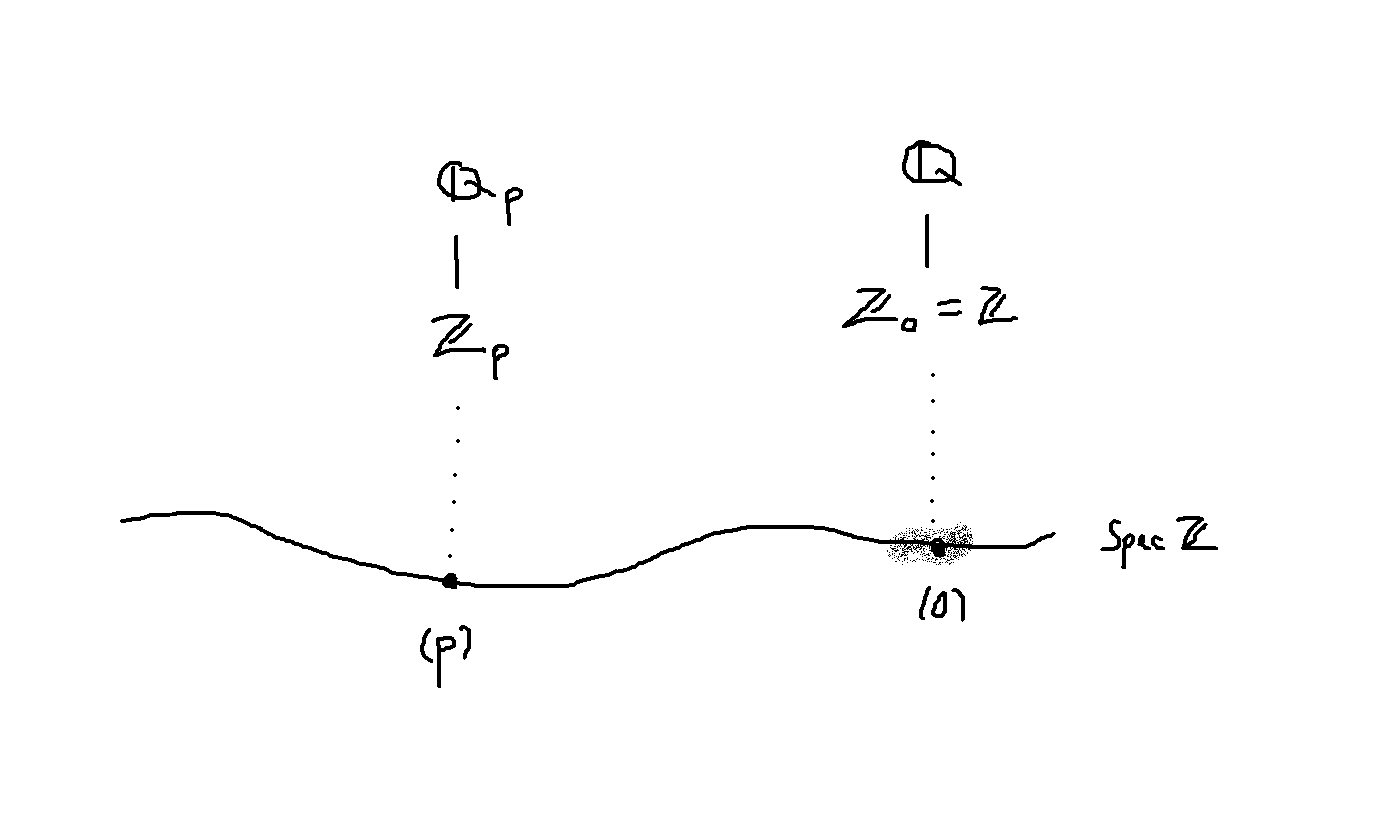
\includegraphics[width=\linewidth,height=\textheight,keepaspectratio]{Figures/places of Spec Z.png}
                            \caption{Places of $\Q$ (note that $(0)$ should be viewed as the generic place-at-infinity).}
                            \label{fig: places_of_Q}
                        \end{figure}
                \end{convention}
                
                \begin{proposition}[Local-global compatibility]
                
                \end{proposition}
                    \begin{proof}
                        
                    \end{proof}
                
                \begin{example}[Places of ramification of more general arithmetic schemes]
                    Below are examples of arithmetic schemes, i.e. schemes over $\Spec \Z$, on which there are primes lying over those of $\Spec \Z$ where ramifications take place.
                        \begin{enumerate}
                            \item \textbf{(The prime spectrum of the ring of integers of a number field):} Consider the following setting:
                                $$
                                    \begin{tikzcd}
                                    	{\Q(\sqrt{d})} & {\Z[\sqrt{d}]} \\
                                    	\Q & \Z
                                    	\arrow[no head, from=2-1, to=1-1]
                                    	\arrow[no head, from=2-2, to=1-2]
                                    	\arrow[no head, from=1-1, to=1-2]
                                    	\arrow[no head, from=2-1, to=2-2]
                                    \end{tikzcd}
                                $$
                            wherein we are consider the quadratic extension $\Q(\sqrt{d})/\Q$ along with the induced integral extension of Dedekind domains $\Z[\sqrt{d}]/\Z$; particularly, let us pick a prime ideal $\p$ of $\Z$ (i.e. either the zero ideal or an ideal generated by a prime number $p$). Now, do the primes of $\Z[\sqrt{d}]$ indeed lie over those of $\Z$ ? First of all, we will need to see what the prime ideals of $\Z[\sqrt{d}]$ actually look like, and luckily, we can apply corollary \ref{coro: prime_splitting_finite_extensions} to do this:
                                \begin{enumerate}
                                    \item Of course, the ideal $(0)\Z[\sqrt{d}]$ is just the zero ideal, and thus admits the trivial factorisation $(0) = (0)$. Because of this, let us only consider non-zero prime ideals of $\Z$ from now on.
                                    \item Then, there are three cases, according to corollary \ref{coro: ramification_quadratic_fields}:
                                        \begin{enumerate}
                                            \item 
                                            \item
                                            \item
                                        \end{enumerate}
                                \end{enumerate}
                            \item \textbf{(A conic over $\Spec \Z$):}
                            \item \textbf{(The line with double origin over $\Spec \Z$):}
                        \end{enumerate}
                    \end{example}
                    
            \subsubsection{Unramfied morphisms}
                \begin{definition}[Unramified morphisms] \label{def: unramified_morphisms}
                    A ring map is said to be \textbf{unramified} if it is of finite type and if the corresponding module of K\"ahler differentials is zero. 
                \end{definition}
                \begin{example}
                    \noindent
                    \begin{itemize}
                        \item \textbf{(\'Etale morphisms):} \'Etale morphisms (cf. definition \ref{def: etale_morphisms}) are trivially unramified. The converse statement is not necessarily true, since there are morphisms of finite type that are not of finite presentation, which is a necessary condition for \'etale-ness (or even just smoothness for that matter).
                        
                        As a concrete example, take any unramified finite extension $E/F$ (cf. definition \ref{def: ramification_indices}), and in the event that these fields have rings of integers (cf. example \ref{example: ring_of_integers}), the induced map:
                            $$\Spec E^{\circ} \to \Spec F^{\circ}$$
                        will also be unramified (in fact, they will be \'etale, since finite extensions come from finite presentations). As a result, for some fixed base scheme $S$, one can think of unramified morphisms $X \to S$ as coming from $S$-schemes $X$ such that preimages of points of $S$ consists merely of a single point. 
                        \item \textbf{(A counter example: non-\'etale smooth morphisms):} A smooth morphism of non-zero relative dimension can not be unramified, since its associated module of K\"ahler differential is not zero. 
                    \end{itemize}
                \end{example}
                
                \begin{proposition}[Locality of ramification] \label{prop: locality_of_ramification}
                    We say that 
                \end{proposition}
                
            \subsection{\'Etale morphisms} \label{subsection: etale_morphisms}
            \begin{definition}[\'Etale morphisms] \label{def: etale_morphisms} \index{\'Etale-ness}
                An \'etale ring map is a smooth ring map whose cotangent complex is quasi-isomorphic to the zero complex. Equivalently, a ring homomorphism is \'etale if and only if it is smooth and of relative dimension $0$ (see proposition \ref{prop: smoothness_implies_almost_finiteness_of_cotangent_complex} for an explanation). 
            \end{definition}
            
            \begin{proposition}[The separable extension criterion for \'etale-ness] \label{prop: separable_criterion_for_etaleness} \index{\'Etale-ness! Separability Criterion}
                Let $\pi: F \to B$ be a ring map of finite presentation. Then, the following statements are equivalent:
                    \begin{enumerate}
                        \item $\pi$ is \'etale.
                        \item The field extension $\kappa_{\pi^{-1}(\q)}/\kappa_{\q}$ of the residue field at $\pi^{-1}(\q) \in |\Spec k|$ over that at $\q \in |\Spec B|$ is separable (and necessarily finite, as \'etale maps are \textit{a priori} of finite presentation) for all $\q \in |\Spec B|$. Note that the extension $\kappa_{\pi^{-1}(\q)}/\kappa_{\q}$ exists thanks to the fact that the stalk map:
                            $$\calO_{\Spec F, \pi^{-1}(\q)} \to \calO_{\Spec B, \q}$$
                        which is actually just: 
                            $$F_{\pi^{-1}(\q)} \to B_{\q}$$
                        is required to be a local homomorphism between local rings.
                        \item If $F$ is a field, then $B$, when viewed as an $F$-vector space, can be written as a (necessarily finite) direct sum of (necessarily finite) separable extensions of $F$ (of course, this assertion is only equivalent to the other two in the event that they are considered with $F$ a field as well).
                    \end{enumerate}
            \end{proposition}
                \begin{proof}
                    This is trivial when $\chara \kappa_{\q} = 0$, as every extension in characteristic $0$ is \textit{a priori} separable (for a proof, please consult \cite[\href{https://stacks.math.columbia.edu/tag/030Q}{Tag 030Q}]{stacks} and \cite[\href{https://stacks.math.columbia.edu/tag/030N}{Tag 030N}]{stacks}). Thus, let us assume that:
                        $$\chara \kappa_{\q} = p$$
                    for some prime $p$. Also, note that the extension $\kappa_{\pi^{-1}(\q)}/\kappa_{\q}$ decomposes into a separable part $\kappa_{\q}^{\sep}/\kappa_{\q}$ (with $\kappa_{\q}^{\sep}$ is the separable closure of $\kappa_{\q}$ inside $\kappa_{\pi^{-1}(\q)}$) and a purely inseparable part $\kappa_{\pi^{-1}(\q)}/\kappa_{\q}^{\sep}$ in the following manner \cite[\href{https://stacks.math.columbia.edu/tag/030K}{Tag 030K}]{stacks}:
                        $$
                            \begin{tikzcd}
                            	{\kappa_{\pi^{-1}(\q)}} \\
                            	{\kappa_{\q}^{\sep}} \\
                            	{\kappa_{\q}}
                            	\arrow[no head, from=3-1, to=2-1]
                            	\arrow[no head, from=2-1, to=1-1]
                            \end{tikzcd}
                        $$
                    \begin{enumerate}
                        \item 
                            \begin{enumerate}
                                \item \textbf{(1 implies 2):} Suppose firstly that \textbf{1} holds, i.e. that $\pi: F \to B$ is \'etale. According to definition \ref{def: etale_morphisms}, this tells us that $B$ is a smooth $F$-algebra that is of relative dimension $0$; in other words, we can write $B$ as $\frac{F[x_1, ..., x_n]}{(f_1, ..., f_n)}$ for some natural number $n$. Now, fix an arbitrary prime ideal $\q \in \left|\Spec \frac{F[x_1, ..., x_n]}{(f_1, ..., f_n)}\right|$, which should be noted to be nothing but a prime of $F[x_1, ..., x_n]$ containing the ideal $(f_1, ..., f_n)$, and note that:
                                    $$\left(\frac{F[x_1, ..., x_n]}{(f_1, ..., f_n)}\right)_{\q} \cong \frac{F[x_1, ..., x_n]_{\q}}{(f_1, ..., f_n)}$$
                                thanks to the fact that colimits commute. Now, let us suppose for the sake of deriving a contradiction, that $\kappa_{\pi^{-1}(\q)}/\kappa_{\q}$ is not a (finite) separable extension for our chosen prime $\q$, and observe that according to the preliminary discussion, this is the same as supposing that the purely inseparable extension $\kappa_{\pi^{-1}(\q)}/\kappa_{\q}^{\sep}$ is non-trivial. 
                                \item \textbf{(2 implies 1):} On the other hand, let us use \textbf{2} as our starting point. 
                            \end{enumerate}
                        \item 
                            \begin{enumerate}
                                \item \textbf{(2 implies 3):} Now, suppose that \textbf{2} is true and that $F$ is a field. Immediately, one sees that:
                                    $$\kappa_{\pi^{-1}{\q}} \cong \calO_{\Spec F, \pi^{-1}(\q)} \cong F_{\pi^{-1}(\q)} \cong F_{(0)} \cong F$$ 
                                which means that $F/\kappa_{\q}$ is a (finite) separable extension for all primes $\q \in \left|\Spec B\right|$. Also, thanks to the hypothesis whereby $F$ is a field, one can write the finitely presented $F$-algebra $B$ as some finite direct some of copies of $F$ (since algebras are first and foremost modules, and modules over fields are vector spaces, which are \textit{a priori} all free). Thus, the \'etale $F$-algebra $B$, when viewed as a vector space over $F$, can written as a finite direct sum of the finite separable extension $F$ of $\kappa_{\q}$, for all $\q \in |\Spec B|$. In other words, \textbf{2} implies \textbf{3}. 
                                \item \textbf{(3 implies 2):} Conversely, suppose that \textbf{3} is true, specifically that:
                                    $$B \cong F^{\oplus d}$$
                                for some natural number $d$, and suppose that the $F$-algebra of finite presentation $B$ is of the form $\frac{F[x_1, ..., x_N]}{(f_1, ..., f_n)}$, for some pair of natural numbers $n, N$. 
                            \end{enumerate}
                        Thus, we have managed to show that \textbf{1} is equivalent to \textbf{2}, and that \textbf{2} is in turn equivalent to \textbf{3}, and thus the three are jointly equivalent. 
                    \end{enumerate}
                \end{proof}
            \begin{corollary}[Finite separable extensions are \'etale] \label{coro: finite_separable_extensions_are_etale}
                Let $k$ be a field and let $B$ be a $k$-algebra of finite presentation. According to proposition \ref{prop: separable_criterion_for_etaleness}, $B$ is \'etale over $k$ if and only if when it is viewed as a $k$-vector space, $B$ is a direct sum of copies of some finite separable extension $K$ over $k$. But $K$ itself is a $k$-algebra, and thus every finite and separable field extension is an \'etale ring map. In fact, it is even better: via the adjoint equivalence:
                    $$
                        \begin{tikzcd}
                        	{{}^{k/}\Comm\Alg^{\op}} & {\Sch^{\aff}_{/\Spec k}}
                        	\arrow[""{name=0, anchor=center, inner sep=0}, "\Spec"', shift right=2, from=1-1, to=1-2]
                        	\arrow[""{name=1, anchor=center, inner sep=0}, "\Gamma"', shift right=2, from=1-2, to=1-1]
                        	\arrow["\dashv"{anchor=center, rotate=-90}, draw=none, from=1, to=0]
                        \end{tikzcd}
                    $$
                any non-empty collection of finite separable extension $\{k \to K_{\alpha}\}_{\alpha \in A}$ of some given ground field $k$ corresponds to an \'etale covering sieve $\{\Spec K_{\alpha} \to \Spec k\}_{\alpha}$ (because spectra of fields are singletons, the joint surjection of presheaves:
                    $$
                        \begin{tikzcd}
                        	{\left(\coprod_{\alpha \in A} h_{\Spec K_{\alpha}}\right) \x_{h_{\Spec k}} \left(\coprod_{\alpha \in A} h_{\Spec K_{\alpha}}\right)} & {\coprod_{\alpha \in A} h_{\Spec K_{\alpha}}} & {h_{\Spec k}}
                        	\arrow["{\pr_2}"', shift right=2, from=1-1, to=1-2]
                        	\arrow["{\pr_1}", shift left=2, from=1-1, to=1-2]
                        	\arrow[dashed, from=1-2, to=1-3]
                        \end{tikzcd}
                    $$
                exists for all non-empty indexing sets $A$). In turn, this implies something remarkable, which is that for all Galois extensions $K/k$ (which are necessarily separable by definition, and hence \'etale) and for all \textit{sheaves} $\calF$ on ${}^{k/}\Comm\Alg^{\op, \petit}_{\et}$ (we refer the reader to paragraph \ref{paragraph: etale_descent} for the descent theory along \'etale morphisms) we have via the fact that finite colimits (in this case, the orbit space ) commute with filtered limits that and the Fundamental Theorem of Galois Theory that:
                    $$
                        \begin{aligned}
                            F(\Spec K)/\Gal(K/k) & \cong \calF(\Spec E)/\left(\underset{E}{\lim} \Aut(E/k)\right)
                            \\
                            & \cong \underset{E}{\lim} \left(\calF(\Spec E)/\Aut(E/k)\right)
                            \\
                            & \cong \underset{E}{\lim} \left(\calF(\Spec k)/\Aut(E/k)\right)
                        \end{aligned}
                    $$
                wherein the limit is the filtered limit taken over the poset of finite separable subextensions $E/k$ of $K/k$; also, note that:
                    $$\calF(\Spec E) \cong \calF(\Spec k)$$
                for all finite separable extensions $E/k$ because sheaves satisfy descent, by definition.
            \end{corollary}
            \begin{remark}[Fibres over rational points of \'etale morphisms and inertia of primes] \label{remark: fibres_of_etale_maps_over_points}
                Let $k$ be a field and let $B$ be an \'etale $k$-algebra. From proposition \ref{prop: separable_criterion_for_etaleness}, we know that there exists a natural number $d$ such that:
                    $$B \cong K^{\oplus d} \cong (k^{\oplus [K : k]})^{\oplus d} \cong k^{\oplus ([K : k] \cdot d)}$$
                as $k$-vector spaces, where $K/k$ is some finite separable extension. Then, thanks to the fact that direct sums of algebra objects in the category ${}_k\Vect$ of $k$-vector spaces are merely products in the commutative algebra category ${}^{k/}\Comm\Alg$, and by employing the adjoint equivalence:
                    $$
                        \begin{tikzcd}
                        	{{}^{k/}\Comm\Alg^{\op}} & {\Sch^{\aff}_{/\Spec k}}
                        	\arrow[""{name=0, anchor=center, inner sep=0}, "\Spec"', shift right=2, from=1-1, to=1-2]
                        	\arrow[""{name=1, anchor=center, inner sep=0}, "\Gamma"', shift right=2, from=1-2, to=1-1]
                        	\arrow["\dashv"{anchor=center, rotate=-90}, draw=none, from=1, to=0]
                        \end{tikzcd}
                    $$
                one gets:
                    $$\Spec B \cong \Spec \prod_{i = 1}^d K \cong \coprod_{i = 1}^d \Spec K$$
                wherein the coproduct is taken in the category of locally ringed spaces over $\Spec k$, but lands in the category of affine schemes (also over $\Spec k$). Lastly, because spectra of fields are singletons, the \'etale $k$-algebra $B$ is nothing but a collection of $d$ disjoint points lying over the single point of $\Spec k$. 
                
                One implication of this is that given any scheme $X$ over $\Spec k$, its fibres over $k$-rational points $x \in X(k)$ are nothing but finite collections of points (even if the fibre is not affine, its affine patches would still necessarily be finite collections of points, as shown above, and thus the whole fibre would be so as well).
            \end{remark}
            
            \begin{definition}[Local isomorphisms and maps identifying local rings] \label{def: local_isomorphisms_and_maps_identifying_local_rings}
                This was taken almost \textit{verbatim} from \cite[\href{https://stacks.math.columbia.edu/tag/096E}{Tag 096E}]{stacks}.
                \begin{enumerate}
                    \item \textbf{(Local isomorphisms):} A ring map:
                        $$\pi: A \to B$$
                    is called a \textbf{local isomorphism} if and only if for all primes $\q \in |\Spec B|$, there exists an element $g \in B$ not contained in $\q$ (i.e. a basic Zariski open neighbourhood $D_B(g)$ of $\q$) such that the \say{restricted} morphism of affine schemes $\pi_g: \Spec B_g \to \Spec A$ fitting into the following commutative diagram in $\Sch^{\aff}$ (the dashed arrow):
                        $$
                            \begin{tikzcd}
                            	{\Spec B_g} & {\Spec B} \\
                            	{} & {\Spec A}
                            	\arrow["\pi", from=1-2, to=2-2]
                            	\arrow["{\lambda_{g, B}}", hook, from=1-1, to=1-2]
                            	\arrow["{\pi_g}"', dashed, from=1-1, to=2-2]
                            \end{tikzcd}
                        $$
                    (wherein $\lambda_{g, B}: B \to B_g$ is the canonical localisation map) is an open immersion.
                    
                    One might also rephrase this definition so it would appear more topological. To that end, observe that having an element $g \in B$ such that $\q \not \ni g$ is actually the same as having a point $\q \in |\Spec B|$ inside a Zariski-open neighbourhood $D_B(g)$, which also happens to be a basic Zariski-open subset of $|\Spec B|$. Also, note that there is a homeomorphism:
                        $$D_B(g) \cong |\Spec B_g|$$
                    Thus, a morphism of affine schemes:
                        $$\pi: \Spec B \to \Spec A$$
                    is a local isomorphism if and only if for all prime ideals $\q$ of $B$, one can identify Zariski-open neighbourhoods of $\pi(\q)$ inside $|\Spec A|$ with basic Zariski-open neighbourhoods of $\q$ inside $|\Spec B|$. 
                    \item \textbf{(Maps identifying local rings):} A ring map:
                        $$\pi: A \to B$$
                    is said to \textbf{identify local rings} (read: to be a \say{local homeomorphism}) if for all $\q \in |\Spec B|$, the canonical arrow:
                        $$\pi_{\q}: \Spec B_{\q} \to \Spec A_{\pi^{-1}(\q)}$$
                    is an isomorphism. Note that this is actually the stalk map at $\q$:
                        $$\pi^{\sharp}_{\q}: \calO_{\Spec A, \pi(\q)} \to \calO_{\Spec B, \q}$$
                    (see corollary \ref{coro: structure_sheaf_properties} for an explanation of why this is the case).
                \end{enumerate}
            \end{definition}
            
            \begin{example}[An \'etale map that is not a local isomorphism of schemes]
                Let $k$ be a field of prime characteristic $p > 2$, and let:
                    $$\pi: \Spec k[u]_u \to \Spec k[t]$$
                be the morphism of affine schemes induced by the ring homomorphism from $k[t]$ to $k[u]_u$ given by:
                    $$t \mapsto u^2$$
                This is an \'etale map, but not a local isomorphism.
                    \begin{enumerate}
                        \item \textbf{(\'Etale-ness):} Let us abuse notations somewhat denote the ring map corresponding to:
                            $$\pi: \Spec k[u]_u \to \Spec k[t]$$
                        by:
                            $$\pi: k[t] \to k[u]_u$$
                        Because this ring homomorphism is specified by the rule:
                            $$t \mapsto u^2$$
                        its image can be thought of as being isomorphic to $k[t, u]_u/(u^2 - t)$, which in turn is isomorphic to $\frac{k[t][u, u']}{(u^2 - t, uu' - 1)}$. Then, let us apply the Jacobian Criterion to check whether or not this is smooth as a $k[t]$-algebra:
                            $$
                                \begin{aligned}
                                    \det \Jac_{u, u'} (u^2 - t, uu' - 1)^T & = \det (\nabla_{u, u'} (u^2 - t), \nabla_{u, u'} (uu' - 1))^T
                                    \\
                                    & = \det
                                        \begin{pmatrix}
                                            \del_u (u^2 - t) & \del_{u'} (u^2 - t)
                                            \\
                                            \del_u (uu' - 1) & \del_{u'} (uu' - 1)
                                        \end{pmatrix}
                                    \\
                                    & = \det
                                        \begin{pmatrix}
                                            2u & 0
                                            \\
                                            u' & u
                                        \end{pmatrix}
                                    \\
                                    & = 2u^2
                                \end{aligned}
                            $$
                        Because $2u^2$ is necessarily inverible in $k[u]_u$, the above tells us that the Jacobian is invertible, and as stated, implies that the image of $\pi$ in $k[u]_u$ is smooth over $k[t]$. Additionally, it is not hard to see that the relative dimension over $k[t]$ of $\frac{k[t][u, u']}{(u^2 - t, uu' - 1)}$ is $2 - 2 = 0$. Thus, the morphism of affine schemes:
                            $$\pi: \Spec k[u]_u \to \Spec k[t]$$
                        specified by $t \mapsto u^2$ is smooth and of relative dimension $0$, which according to definition \ref{def: etale_morphisms}, means that it is \'etale. One can imagine this morphism as follows:
                            \begin{figure}[H]
                                \centering
                                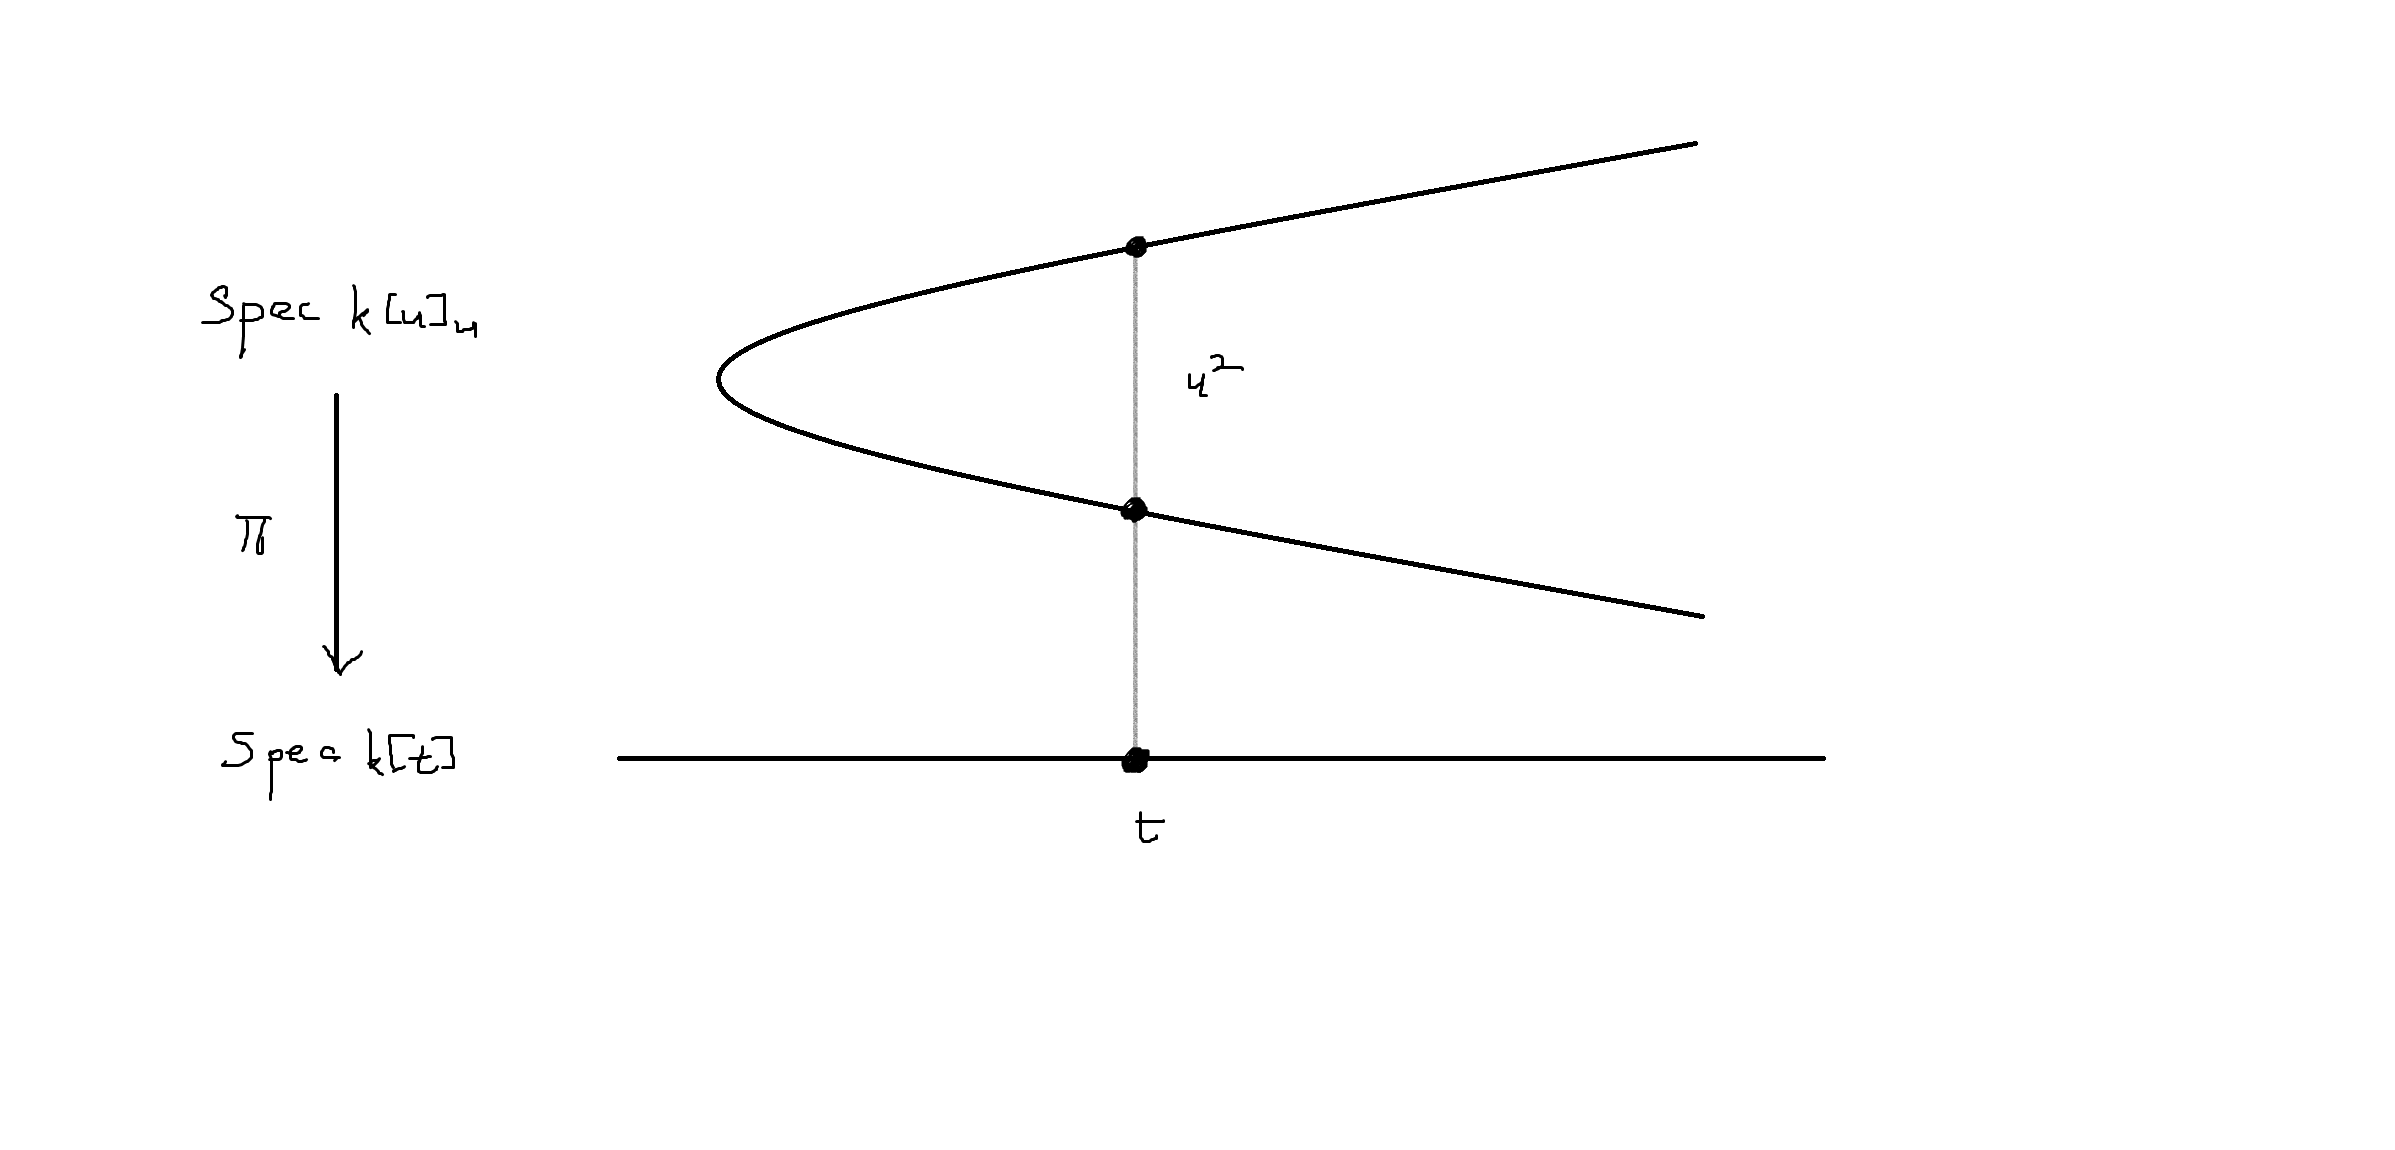
\includegraphics[width=\linewidth,height=\textheight,keepaspectratio]{Figures/etale_but_not_locally_isomorphic.png}
                                \caption{A morphism that, while \'etale, is not a local isomorphism.}
                                \label{fig: etale_but_not_locally_isomorphic}
                            \end{figure}
                        and it should be clear how the preimage of \say{points} in $\Spec k[t]$, by virtue of being disjoint pairs of \say{points} in $\Spec k[u]_u$, are zero-dimensional.
                        \item \textbf{(Failure to be a local isomorphism):} First of all, recall that the image of the ring homomorphism:
                            $$\pi: k[t] \to k[u]_u: t \mapsto u^2$$
                        is $\frac{k[t][u, u']}{(u^2 - t, uu' - 1)}$, as shown above. Because of this, to show why the above ring map fails to be a local isomorphism, it shall suffice, according to definition \ref{def: local_isomorphisms_and_maps_identifying_local_rings}, to find a Zariski-open neighbourhood of some prime ideal $\q$ of $\frac{k[t][u, u']}{(u^2 - t, uu' - 1)}$ (which we might as well take to be a basic Zariski-open subset $D_{\frac{k[t][u, u']}{(u^2 - t, uu' - 1)}}(g)$) such that the dashed arrow in the following commutative diagram is \textit{not} an open immersion:
                            $$
                                \begin{tikzcd}
                                	{\Spec \frac{k[t]\left[u, u', \frac1g\right]}{(u^2 - t, uu' - 1)}} && {\Spec \frac{k[t][u, u']}{(u^2 - t, uu' - 1)}} \\
                                	& {} & {\Spec k[t]}
                                	\arrow["\pi", from=1-3, to=2-3]
                                	\arrow["{\lambda_{g, \frac{k[t][u, u']}{(u^2 - t, uu' - 1)}}}", hook, from=1-1, to=1-3]
                                	\arrow["{\pi_g}"', dashed, from=1-1, to=2-3]
                                \end{tikzcd}
                            $$
                        wherein
                            $$\lambda_{g, \frac{k[t][u, u']}{(u^2 - t, uu' - 1)}}: \frac{k[t][u, u']}{(u^2 - t, uu' - 1)} \to \frac{k[t]\left[u, u', \frac1g\right]}{(u^2 - t, uu' - 1)}$$
                        is the canonical localisation map; also, note that:
                            $$D_{\frac{k[t][u, u']}{(u^2 - t, uu' - 1)}}(g) \cong \left|\Spec \frac{k[t]\left[u, u', \frac1g\right]}{(u^2 - t, uu' - 1)}\right|$$
                        To that end, let us first rewrite $\Spec k[t]$ as $\Spec \frac{k[t][u, u']}{(u, u')}$. Then, notice that the ideal $(u, u')$ of $k[t][u, u']$ admits the ideal $(u^2 - t, uu' - 1)$ (also of $k[t][u, u']$) as a submodule, as the latter is spanned by all $k[t][u, u']$-linear combinations of $u$ and $u'$, which include both $u^2 - t$ and $uu' - 1$. By applying the Third Isomorphism Theorem, which allows us to write down the following isomorphisms of $k[t][u, u']$-modules:
                            $$k[t] \cong \frac{k[t][u, u']}{(u, u')} \cong \frac{k[t][u, u']/(u^2 - t, uu' - 1)}{(u, u')/(u^2 - t, uu' - 1)}$$
                        From this, one can infer that prime ideals of $\frac{k[t][u, u']}{(u^2 - t, uu' - 1)}$ are precise;y those of $\frac{k[t][u, u']}{(u, u')}$ that are inside $(u^2 - t, uu' - 1)$, which themselves are prime ideals of $k[t][u, u']$ (read: $k[t, u, u']$) that are contained in both $(u^2 - t, uu' - 1)$ and $(u, u')$, and as the latter contain the former, these are primes of $k[t][u, u']$ that are contained in $(u^2 - t, uu' - 1)$. The primes of $\frac{k[t]\left[u, u', \frac1g\right]}{(u^2 - t, uu' - 1)}$ are therefore just primes of $k[t][u, u']$ that are contained in $(u^2 - t, uu' - 1)$ and do not contain some chosen element $g$ of $\frac{k[t]\left[u, u'\right]}{(u^2 - t, uu' - 1)}$. 
                    \end{enumerate}
            \end{example}
    
    \section{\'Etale cohomology for schemes: The Chosen One} 
        \subsection{Feats and drawbacks of \'etale cohomology}
        
        \subsection{\texorpdfstring{$\ell$}{}-adic cohomology theory}
            \subsubsection{\texorpdfstring{$\ell$}{}-adic cohomology: "This is where the fun begins"}
                Let $X$ be a smooth projective scheme over a base field that is possibly of some prime characteristic $p$. Let $\ell$ be a prime different from $p$. By \say{$\ell$-adic cohomology}, we shall mean the cohomology theory whose cohomology groups are given by:
                    $$H^i_{\Q_{\ell}}(X) \cong \underset{n \in \N}{\lim} H_{\et}^i(X, \Z/\ell^{n + 1}\Z) \tensor_{\Z_{\ell}} \Q_{\ell}$$
                This means, among other things, that $\ell$-adic cohomology is effectively a \say{singular cohomology theory} for (smooth projective) schemes. This, however, is not the only amazing property that $\ell$-adic cohomology enjoys: it is also a Weil cohomology theory (see definition \ref{def: weil_cohomology_theories} for a description of what this means). At surface level, this might seem odd, since only \'etale cohomology with torsion coefficients gives satisfactory results. However, this is precisely why we take the limit over the torsion rings $\Z/\ell^{n + 1}\Z$ and then base change to $\Q_{\ell}$: $\Q_{\ell}$ is a field of characteristic $0$, and hence can serve as the field of a coefficients of a Weil cohomology theory (cf. definition \ref{def: weil_cohomology_theories}). 
                
                To check that $\ell$-adic cohomology is indeed a Weil cohomology theory, let us \say{simply} go through the axioms laid out in definition \ref{def: weil_cohomology_theories}.
            
                \paragraph{Finiteness}
            
                \paragraph{The K\"unneth Formula}
                
                \paragraph{Poincar\'e Duality}
            
                \paragraph{The Lefschetz Conditions}
                
            \subsubsection{The trace formula}
        
            \subsubsection{The Artin comparison theorem: an \'etale GAGA theorem}